\documentclass[11pt,a4paper]{article}
%\usepackage[utf8]{inputenc}
%\usepackage[ascii]{inputenc}
\usepackage[margin=0.7in]{geometry}
%\usepackage{geometry}
\usepackage[dvipsnames]{xcolor}
\usepackage{textcomp}
\usepackage{graphicx}
\usepackage{caption}
\usepackage{subcaption}
\usepackage{amssymb}
\usepackage{amsmath}
\usepackage{tikz}

\begin{document}
\title{Résumé \& Méthodes chapitre VI: Synthèse de filtres numériques}
\maketitle

\section{Définition}
Synthèse de filtre :  Calcul des \textbf{coefficients} de la fonction  de transfert ou de la réponse impulsionnelle de façon à obtenir une réponse correspondant au \textbf{gabarit}

\section{Synthèse de filtres à réponse impulsionnelle finie/non-récursifs}
Les méthodes de synthèse des filtres non-récursifs suivent le principe général suivant  :
\begin{center}
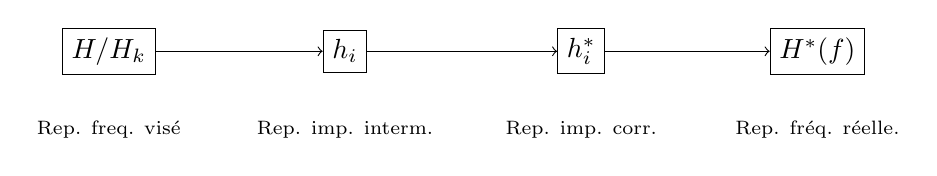
\begin{tikzpicture}
		\node[rectangle,draw,align=center] (I) at (1,0) {$H/H_k$};
		\draw (1,-1) node[text centered] {\scriptsize Rep. freq. visé};
		\node[rectangle,draw,align=center] (D) at (4,0) {$h_i$};
		\draw (4,-1) node[text centered] {\scriptsize Rep. imp. interm.};
		\node[rectangle,draw,align=center] (N) at (7,0) {$h_i^*$};
				\draw (7,-1) node[text centered] {\scriptsize Rep. imp. corr.};
		\node[rectangle,draw,align=center] (B) at (10,0) {$H^*(f)$};	
		\draw (10,-1) node[text centered]{\scriptsize Rep. fréq. réelle.};
		
		\draw[->] (I)--(D);
		\draw[->] (D)--(N);
		\draw[->] (N)--(B);
\end{tikzpicture}
\end{center}

Les méthodes existantes sont distingués par la forme de la réponse en amplitude du spectre, c'est-à-dire la raideur de la transition, l'amplitude des ondulations dans la bande passante et la bande affaiblie. Plus on souhaite contrôler ou contraindre précisément ces paramètres plus les calculs pour arriver à la fonction de transfert souhaités auront tendance à être complexes.

\subsection{Méthodes des fenêtres}
\begin{center}
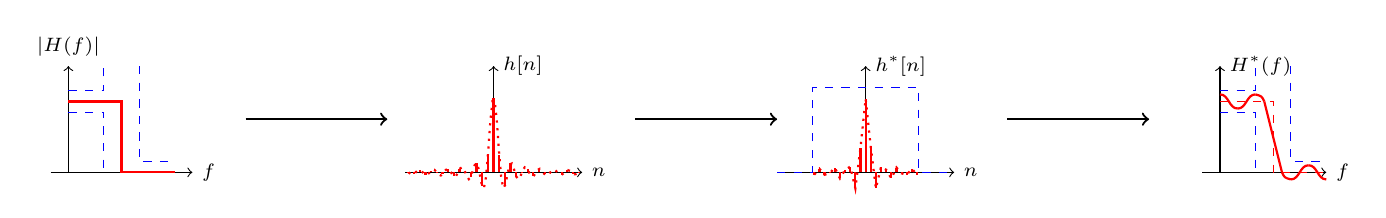
\begin{tikzpicture}
\begin{scope}[scale=0.45]
	\draw[->] (-0.5,0)-- (3.5,0)node[right] {\scriptsize $f$} ;
%\draw (-0.3,-0.3) node {0};
\draw[->] (0,0)-- (0,3)node[above] {\scriptsize $|H(f)|$};


%\draw (3,-0.3) node {$f_e/2$};


\draw[dashed,blue](0,1.7)--(1,1.7)--(1,0);
\draw[dashed,blue](0,2.3)--(1,2.3)--(1,3);
\draw[dashed,blue](2,3)--(2,0.3)--(3,0.3);

	\draw[thick,red]   (0,2)--(1.5,2)--(1.5,0)--(3,0);
	%\draw[->,thick] (0.75,-0.5)--(0.75,-1);
	%\draw (1.5,-0.3) node {$f_e/4$};
	\draw[->,thick] (5,1.5)--(9,1.5);
\end{scope}



\begin{scope}[scale=0.45,xshift=12cm]
%\draw[->,thick] (0,4)--(0,3.4);
\draw[->] (-2.5,0)-- (2.5,0) node[right]{\scriptsize $n$};
%\draw (0,-0.3) node {0};
\draw[->] (0,0)-- (0,3)node[right]{\scriptsize $h[n]$};

\draw[dotted,thick, domain=-2.4:2.4,color=red,samples=80] plot (\x,{120*sin(5*3.14*\x r  )/(5*3.14*\x r)});
\draw[thick, domain=-2.4:2.4,color=red,samples=31] plot [ycomb] (\x,{120*sin(5*3.14*\x r  )/(5*3.14*\x r)});
\draw[->,thick] (4,1.5)--(8,1.5);
\end{scope} 



\begin{scope}[scale=0.45,xshift=22.5cm]
\draw[->] (-2.5,0)-- (2.5,0) node[right]{\scriptsize $n$};
%\draw (0,-0.3) node {0};
\draw[->] (0,0)-- (0,3)node[right]{\scriptsize $h^*[n]$};

\draw[dotted,thick, domain=-1.45:1.45,color=red,samples=21] plot (\x,{120*sin(5*3.14*\x r  )/(5*3.14*\x r)});
\draw[thick, domain=-1.45:1.45,color=red,samples=21] plot [ycomb] (\x,{120*sin(5*3.14*\x r  )/(5*3.14*\x r)});


		\draw[dashed,blue] (-2.5,0)--(-1.5,0)--(-1.5,2.4)--(1.5,2.4)--(1.5,0)--(2.5,0);
		
		\draw[->,thick] (4,1.5)--(8,1.5);
		\end{scope}
		
		%\draw[->,thick] (26,1)--(31,1);
		
		\begin{scope}[scale=0.45,xshift=32.5cm]
	\draw[->] (-0.5,0)-- (3,0)node[right] {\scriptsize $f$};
%\draw (0,-0.5) node {0};
\draw[->] (0,0)-- (0,3) node[right] {\scriptsize $H^*(f)$};


\draw[dashed,red]   (0,2)--(1.5,2)--(1.5,0)--(3,0);

%ondulations BP
 \draw[thick,red] (0,2.2) .. controls (0.25,2.2)  and (0.25,1.8)  .. (0.5,1.8);
  \draw[thick,red] (0.5,1.8) .. controls (0.75,1.8)  and (0.75,2.2)  .. (1,2.2);
   \draw[thick,red] (1,2.2) .. controls (1.18,2.15) and (1.18,2.15)  .. (1.25,2);


%(1.5,2.1) and (1.2,2.1) 

%droite descendant de 1 à 0
\draw[thick,red] (1.25,2)--(1.75,0);
  
\draw[dashed,blue](0,1.7)--(1,1.7)--(1,0);
\draw[dashed,blue](0,2.3)--(1,2.3)--(1,3);
\draw[dashed,blue](2,3)--(2,0.3)--(3,0.3);
 
%ondulations BA
  \draw[thick,red] (2,-0.2) .. controls (2.25,-0.2)  and (2.25,0.2)  .. (2.5,0.2);
 \draw[thick,red] (2.5,0.2) .. controls (2.75,0.2)  and (2.75,-0.2)  .. (3,-0.2);
    \draw[thick,red] (1.75,0) .. controls (1.82,-0.15) and (1.82,-0.15)  .. (2,-0.2);
    
\end{scope}
\end{tikzpicture}
\end{center}

\vspace{0.2cm}
\begin{enumerate}
\item Réponse en fréquence de filtre idéal 
\vspace{0.2cm}
\item Réponse impulsionnelle idéale 
\vspace{0.2cm}
\item Fenêtrage $\rightarrow$ réponse impulsionnelle réelle 
\vspace{0.2cm}
\item Réponse en fréquence réelle
\end{enumerate}
\vspace{0.3cm}
\underline{Ce qu'il faut bien comprendre}:
\begin{itemize} 
\item \textbf{Filtre idéal} $\rightarrow$ \textbf{Réponse impulsionnelle infinie}
\item \textbf{Fenêtrage} $\rightarrow$ \textbf{Ondulations} 
\end{itemize}

Les diffférentes fenêtres permettent de "régler" le niveau d'ondulations et la selectivité du filtre. La \textbf{fenêtre de Hamming} est celle qui permet d'avoir le moins d'oscillations pour une sélectivité donnée

\newpage
\subsection{Méthodes de l'échantillonnage en fréquence}
\begin{center}
\begin{tikzpicture}
	\begin{scope}[scale=0.8]
	\draw[->] (-0.5,0)-- (3.5,0)node[right] {\scriptsize $f$} ;
%\draw (-0.3,-0.3) node {0};
\draw[->] (0,0)-- (0,3)node[above] {\scriptsize $H_k$};

\draw[dashed,blue](0,1.7)--(1,1.7)--(1,0);
\draw[dashed,blue](0,2.3)--(1,2.3)--(1,3);
\draw[dashed,blue](2,3)--(2,0.3)--(3,0.3);

	%\draw[thick,red]   (0,2)--(1.5,2)--(1.5,0)--(3,0);
	\draw[->,thick,red] (0,0)--(0,2);
	\draw[->,thick,red] (0.5,0)--(0.5,2);
	\draw[->,thick,red] (1,0)--(1,2);
		\draw[->,thick,red] (1.5,0)--(1.5,1);
	\draw[->,thick,red] (2,0)--(2,0);
	\draw[->,thick,red] (2.5,0)--(2.5,0);
	\draw[->,thick,red] (3,0)--(3,0);
	\draw[->] (4.5,1.5)--(8.5,1.5); 
	\draw (1,-1.5) node[text centered] {\scriptsize Ech. Fréq. visés};
	\end{scope}
	
%	\begin{scope}[scale=0.6,xshift=9.5 cm]
%	\draw[->] (-2,0)-- (2,0)node[right] {\scriptsize $t$} ;
%\draw[->] (0,0)-- (0,3)node[above] {\scriptsize $h_k$};
%\draw[thick,blue] plot coordinates{
%(-6/3,0.006*5)
%(-5/3,0.024*5)
%(-4/3,-0.025*5)
%(-3/3,-0.081*5)
%(-2/3,0.035*5)
%(-1/3,0.31*5)
%(0/3,0.4615*5)
%(1/3,0.31*5)
%(2/3,0.035*5)
%(3/3,-0.081*5)
%(4/3,-0.025*5)
%(5/3,0.024*5)
%(6/3,0.006*5)};
%\draw[->] (2.5,1.5)--(4.5,1.5); 
%\draw (0,-1.5) node[text centered] {\scriptsize Rép. Imp.};
%\end{scope}
	
	\begin{scope}[scale=1.6,xshift=6cm]
\draw[->] (-2.1,0)-- (2.1,0)node[right] {\scriptsize $f$} ;
\draw[->] (0.02,0)-- (0.02,1.5)node[above] {\scriptsize  $|H(f)|$};
\draw[thick,blue] plot file {module_freq_samp.txt};


\draw[->,thick,red] (0+0.02,0)--(0+0.02,1);
\draw[->,thick,red] (0.3077+0.02,0)--(0.3077+0.02,1);
\draw[->,thick,red] (0.6154+0.02,0)--(0.6154+0.02,1);
\draw[->,thick,red] (0.9231+0.02,0)--(0.9231+0.02,0.5);
\draw[->,thick,red] (1.2038+0.02,0)--(1.2038+0.02,0);
\draw[->,thick,red] (1.5385+0.02,0)--(1.5385+0.02,0);
\draw[->,thick,red] (1.8462+0.02,0)--(1.8462+0.02,0);
\draw (0,-0.75) node[text centered] {\scriptsize Rep. Fréq. Réelle};
\end{scope}
	
\end{tikzpicture}
\end{center}

\begin{enumerate}
\item On fixe des valeurs pour le spectre dans les trois régions
\item On interpole la réponse en fréquence à partir des points fixés
\end{enumerate}

Dans la méthode des fenêtres, l'amplitude des oscillations est forcément la même en bande passante et atténuée. Avec la méthode de l'échantillonnage en fréquence on peut avoir des \textbf{amplitudes d'oscillations différentes entre les bandes passantes et affaiblies}.


\subsection{Résumé \& autres méthodes}
Résumons les deux premières méthodes ainsi que d'autres méthodes utilisées couramment pour synthèse de filtres non-récursifs.

\begin{itemize}
\item \textbf{\underline{Méthode des fenêtres}}: Contrôle sur peu de paramètres, oscillations symétriques entre bande passante et affaiblie. 
\item \textbf{\underline{Méthode de l'échantillonnage en fréquence}}: Permet de choisir les points par lesquels passent la réponse en fréquence, mais sinon même caractéristiques que la méthode précédente
\item \textbf{\underline{Méthode des moindres carrés}}: Généralisation de la méthode précédente. Permet d'avoir des amplitudes différentes pour les oscillations en bande-passante et en bande affaiblie
\item \textbf{\underline{Méthode itérative par TFD}}: Est utilisée quand l'amplitude des oscillations sur la bande passante et affaiblie doit être constante.
\item \textbf{\underline{Méthode par approximation de Tchebychev}}: Permet de spécifier complètement le filtre. (amplitude dans chaque bande et largeur de transition)
\end{itemize}

\section{Synthèse de filtres à réponse impulsionnelle infinie/récursifs}
Il existe deux classes de méthodes pour synthétiser des filtres récursifs:
\begin{itemize}
\item Calcul direct des coefficients par fonctions modèles
\item Techniques itératives
\end{itemize}

\subsection{Calcul direct des coefficients par fonctions modèles}
Le principe général des fonctions modèles est de partir d'une fonction analogique avec les caractéristiques souhaitées  avant de le convertir en filtre numérique

\begin{center}
\begin{tikzpicture}
\begin{scope}[scale=2]
\draw[->](0,0)--(0,1) node[above]{$H(s)$};
\draw[->](0,0)--(1,0) node[right]{$s$};
\draw (0.5,-0.5) node[text centered]  {\scriptsize fct° transfert  analogique};


\draw[thick,blue] (0,0.8).. controls(0.9,0.8) and (0.25,0).. (0.9,0);


\draw[->] (1.2,0.5)--(1.7,0.5);
\node[rectangle,draw,align=center] (I) at (3,0.5) {$z= f(s)$};



\draw[->] (4.2,0.5)--(4.7,0.5);

\draw[->](5,0)--(5,1) node[above]{$H(z)$};
\draw[->](5,0)--(6,0) node[right]{$z$};

\draw[thick,red] (5,0.8).. controls(5.9,0.5) and (5.25,0.3).. (5.9,0);
\draw (5.5,-0.5) node[text centered]  { \scriptsize fct° transfert numérique};
\end{scope}
\end{tikzpicture}
\end{center}

La conversion utilisée doit avoir les caractéristiques suivantes : 
\begin{itemize}
\item Fraction rationnelle en $s$ $\rightarrow$ Fraction rationnelle en $z$

\item Filtre stable en  $s$ $\rightarrow$ Filtre stable en  $z$

\item Conservation des propriétés en amplitude (ex: passe-haut $\rightarrow$ passe-haut)
\end{itemize}

Dans le cours, les exemples de l'\textbf{invariance impulsionnelle} et de l'\textbf{approximation de la dérivée} ont été traité pour illustrer les notions Mais elle ne vérifient généralement pas la conservation des propriétés en amplitude. En pratique, c'est donc souvent la \textbf{transformation bilinéaire} qui est utilisée.

\subsubsection{Approximation de la dérivée}
L'approximation de la dérivée se base sur la conversion suivante :
\[\boxed{s  \approx \frac{1-z^{-1}}{T_e}} \]

Cette méthode est simple, mais elle \textbf{génère du repliement spectral} pour les filtres n'ayant pas une amplitude nulle à haute fréquence
\subsubsection{Invariance Impulsionnelle}
La méthode de l'invariance impulsionnelle exprime le fait qu'une manière d'obtenir le filtre récursif numérique est d'\textbf{échantillonner la réponse du filtre analogique visé}.

On part donc du filtre analogique qu'on décompose en éléments simples
\[ H(s)  =  \frac{1+ a_1 s + a_2 s^2 + \cdots + a_n s^m }{1+ b_1 s + b_2 s^2 + \cdots + b_n s^n} = \frac{c_1}{s-p_1} + \frac{c_2}{s-p_2} + \cdots + \frac{c_n}{s-p_n} \]

et l'invariance impulsionnelle permet d'écrire,
\[ H_k(s) = \frac{c_k}{s-p_k} \rightarrow H_k(z)= \frac{c_k}{1-e^{p_k T_e}z^{-1}}\]

\[ H(s) = \frac{1+ a_1 s + a_2 s^2 + \cdots + a_n s^m }{1+ b_1 s + b_2 s^2 + \cdots + b_n s^n}  \] 

\[ \boxed{\rightarrow H(z) = \frac{c_1}{1-e^{p_1 T_e}z^{-1}} + \frac{c_2}{1-e^{p_2 T_e}z^{-1}}  + \cdots + \frac{c_n}{1-e^{p_n T_e}z^{-1}}} \]

Cette méthode a le même défaut que la précédente. Elle ne permet pas forcément de bien transposer tous les comportments en fréquence.

\subsubsection{Transformation bilinéaire}
La transformation bilinéiare est basée sur la conversion suivante :

\[ \boxed{ s = \frac{2}{T_e} \frac{1-z^{-1}}{1+z^{-1}}} \]

Cette conversion remplit tous les critères cités précedemment. Cependant, la relation entre les fréquences analogiques et les fréquences numériques n'est pas linéaire: 

\[ \rightarrow \nu_a = \frac{1}{ \pi T_e} \tan(\pi \nu_n T_e)\]

Cette relation implique que si on part d'un filtre analogique avec une fréquence de coupure $\nu_{c,a}$ que l'on souhaite, alors le filtre numérique aura une fréquence de coupure $\nu_{c,n}$ différentes. Pour cette raison il est nécessaire de \textbf{prédéformer les fréquences du filtre analogique} avant d'appliquer la transformation bilinéaire.

En résumé:
\begin{center}
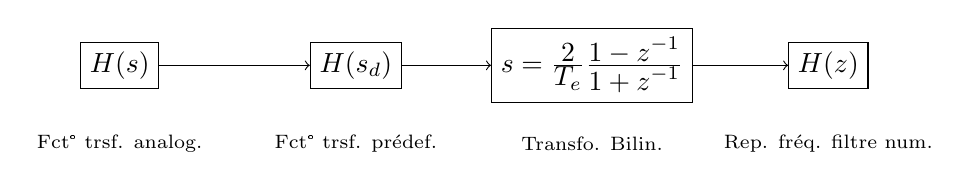
\begin{tikzpicture}
		\node[rectangle,draw,align=center] (I) at (1,0) {$H(s)$};
		\draw (1,-1) node[text centered] {\scriptsize Fct° trsf. analog.};
		\node[rectangle,draw,align=center] (D) at (4,0) {$H(s_d)$};
		\draw (4,-1) node[text centered] {\scriptsize Fct° trsf. prédef.};
		\node[rectangle,draw,align=center] (N) at (7,0) {$s = \frac{\displaystyle  2}{\displaystyle  T_e} \frac{\displaystyle 1-z^{-1}}{\displaystyle  1+z^{-1}}$};
				\draw (7,-1) node[text centered] {\scriptsize Transfo. Bilin.};
		\node[rectangle,draw,align=center] (B) at (10,0) {$H(z)$};	
		\draw (10,-1) node[text centered]{\scriptsize Rep. fréq. filtre num.};
		\draw[->] (I)--(D);
		\draw[->] (D)--(N);
		\draw[->] (N)--(B);
\end{tikzpicture}
\end{center}
\begin{enumerate}
\item On sélectionne une filtre analogique avec les bonnes propriétés en fréquence 
\item On prédéforme les fréquences en analogique avec $\nu_a = \frac{1}{ \pi T_e} \tan(\pi \nu_n T_e)$
\item On applique la transformation bilinéaire
\end{enumerate}


\subsection{Techniques itératives}
Les méthodes itératives sont basées sur le même principe que les méthodes itératives pour les filtres non-récursifs.

\end{document}